\chapter{Thiết kế hệ thống}
\section{Thiết kế giao diện bằng ứng dụng Figma}
\textbf{Thiết kế giao diện trang hiển thị sản phẩm}
\begin{figure}[H]
    \begin{center}
    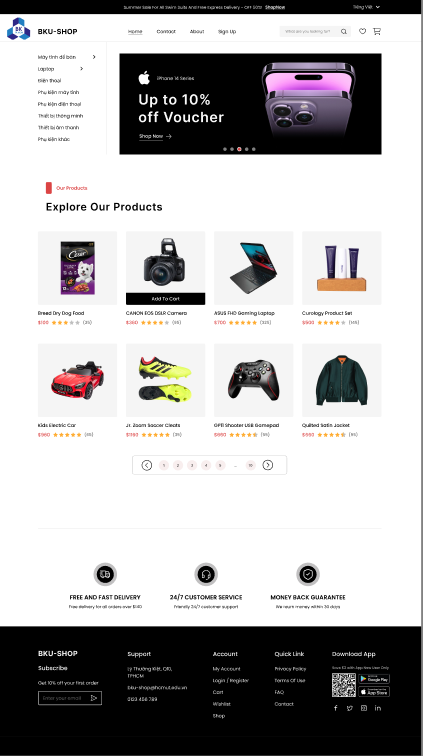
\includegraphics[scale=0.8]{images/hieu/chap-4/display-product-page.png}
    \vspace*{5mm}
    \caption{Thiêt kế giao diện trang hiển thị sản phẩm}
    \end{center}
\end{figure}
\begin{itemize}
    \item \textbf{Phần Header}
    \newline
    Phần đầu trang web gồm các thành phần sau:
    \begin{itemize}
        \item Logo của trang web
        \item Tên trang web
        \item Thanh điều hướng chứa các nút điều hướng đến các trang khác
        \item Ô tìm kiếm sản phẩm
        \item Nút đăng nhập
        \item Giỏ hàng
    \end{itemize}
    \begin{figure}[H]
        \begin{center}
        
\includegraphics[scale=0.5]{images/hieu/chap-4/header.png}
        \vspace*{5mm}
        \caption{Phần đầu trang - Header}
        \end{center}
    \end{figure}

    \item \textbf{Phần Category}
    \newline
    Phần category là một thanh dropdown chứa các danh mục sản phẩm.
    \begin{figure}[H]
        \begin{center}
        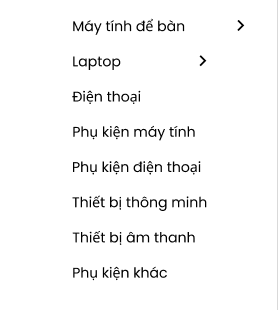
\includegraphics[scale=1]{images/hieu/chap-4/category.png}
        \vspace*{5mm}
        \caption{Phần danh mục sản phẩm - Category}
        \end{center}
    \end{figure}
    \item \textbf{Phần Discount}
    \newline
    Phần discount là một slide chứa các giảm giá của các sản phẩm. Slide sẽ tự chuyển động sau một khoảng thời gian nhất định hoặc có thể chuyển động bằng cách nhấn vào các nút điều hướng.
    \begin{figure}[H]
        \begin{center}
        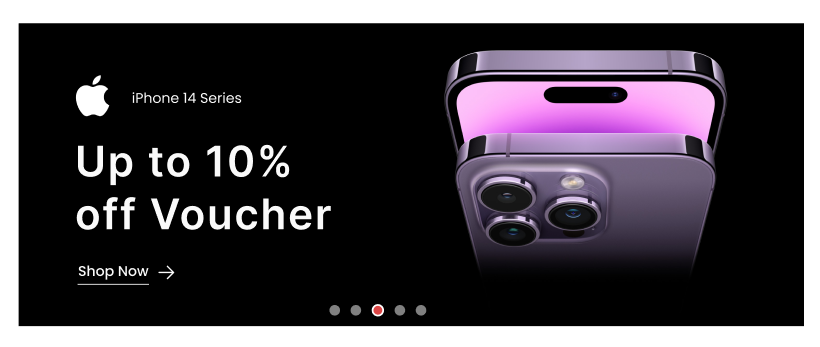
\includegraphics[scale=0.7]{images/hieu/chap-4/discount.png}
        \vspace*{5mm}
        \caption{Phần giảm giá - Discount}
        \end{center}
    \end{figure}
    \item \textbf{Phần Product}
    \newline
    Phần product hiển thị các sản phẩm theo danh mục. Mỗi sản phẩm gồm có:
    \begin{itemize}
        \item Hình ảnh sản phẩm
        \item Tên sản phẩm
        \item Giá sản phẩm
        \item Nút thêm vào giỏ hàng
        \item Nút xem chi tiết sản phẩm
    \end{itemize}
    \begin{figure}[H]
        \begin{center}
        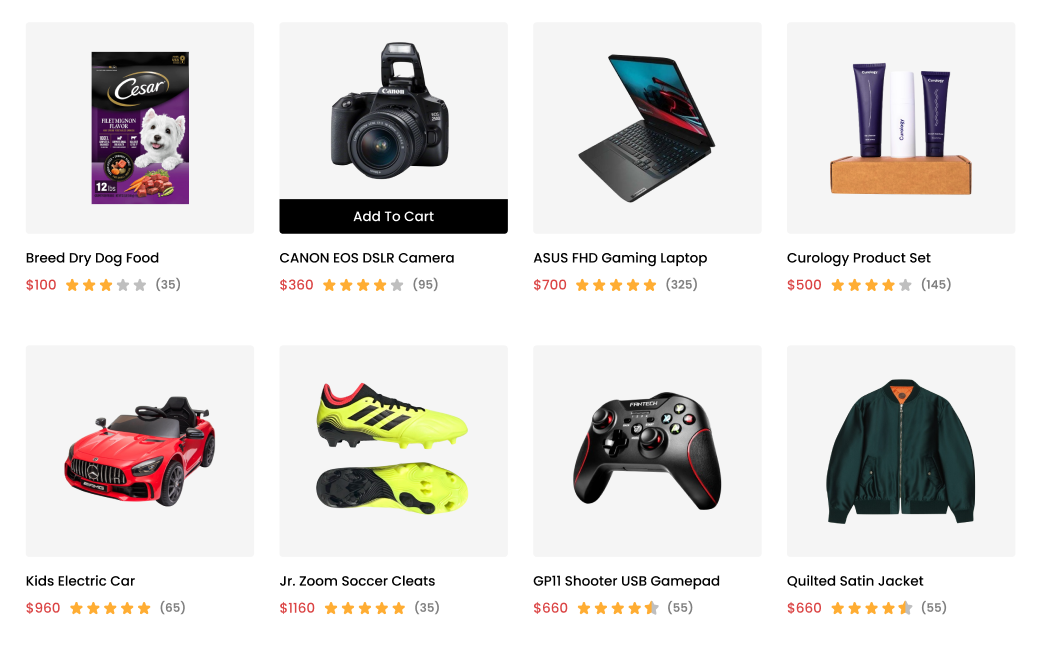
\includegraphics[scale=0.7]{images/hieu/chap-4/product.png}
        \vspace*{5mm}
        \caption{Phần sản phẩm - Product}
        \end{center}
    \end{figure}
    \item \textbf{Phần Footer}
    \newline
    Phần footer là phần cuối trang web chứa các thông tin về trang web, các liên kết đến các trang mạng xã hội, các liên kết đến các trang khác.
    \begin{figure}[H]
        \begin{center}
        
\includegraphics[scale=0.5]{images/hieu/chap-4/footer.png}
        \vspace*{5mm}
        \caption{Phần cuối trang - Footer}
        \end{center}
    \end{figure}
\end{itemize}
\section{Thiết kế kiến trúc}
 \begin{figure}[H]
    \begin{center}
    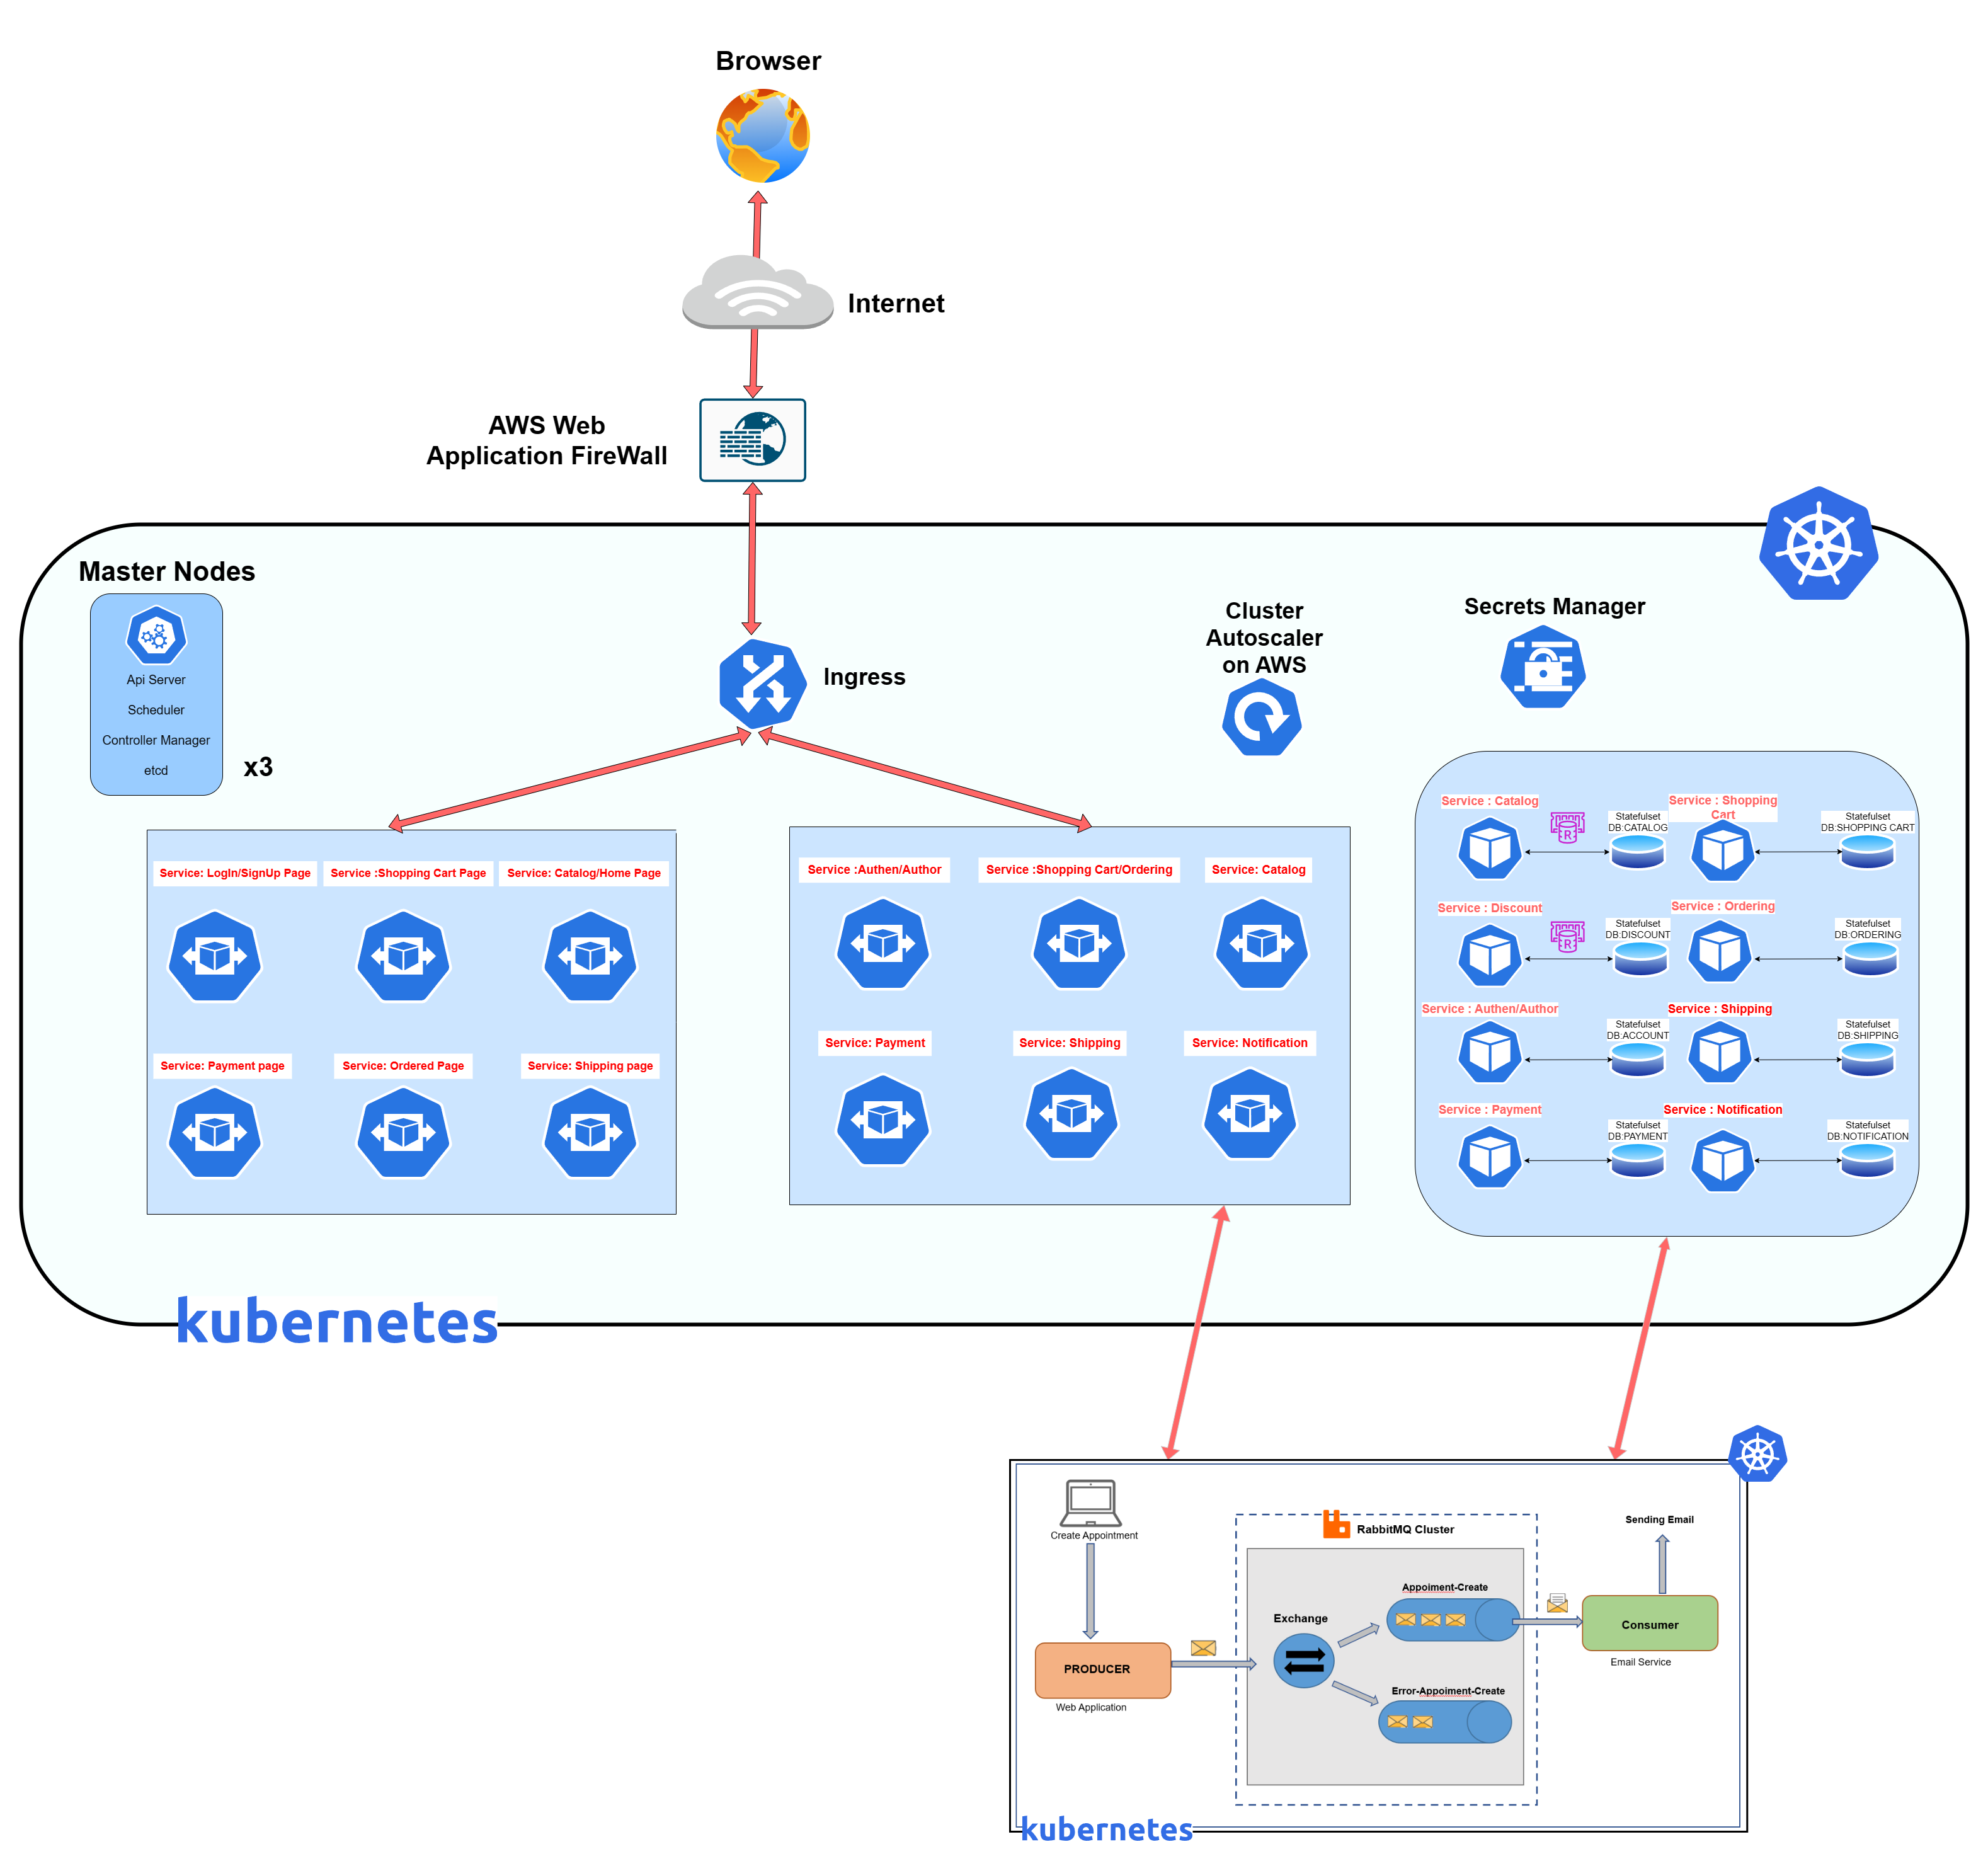
\includegraphics[scale = 0.13]{images/phat/Architech_System.png}
    \vspace*{7mm}
    \caption{System Architecture}
    \end{center}
    \label{}
\end{figure}
\noindent Hệ thống bao gồm 02 cluster: 01 cluster chính để chứa tất cả các service của hệ thống, cluster còn lại dùng để chứa RabbitMQ. Các service bên trong cluster chính được chia thành 03 nhóm chính: fontend, backend, database. Các service frontend và backend có thể được truy cập từ bên ngoài thông qua nginx ingress (reverse proxy, load balancer). Service backend được kết nối tới ingress vì frontend sử dụng client side rendering, các lệnh js được chạy ở browser trên máy của client, do đó cần endpoint để truy cập vào các api backend microservices. Các service ở nhóm backend và nhóm database giao tiếp với nhau thông qua rabbitMQ.
\begin{figure}[H]
    \begin{center}
    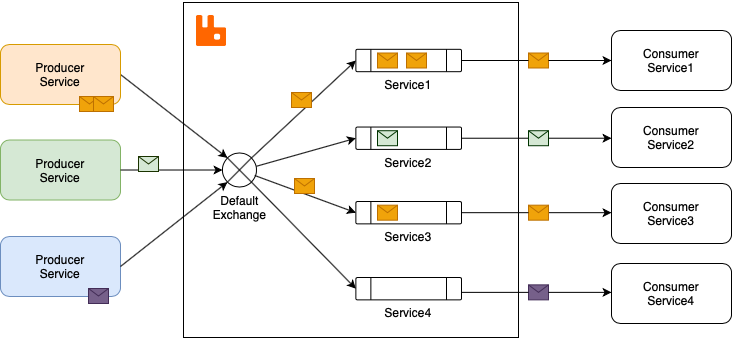
\includegraphics[scale = 0.55]{images/phat/rabbitMQ.png}
    \vspace*{7mm}
    \caption{Rabbit MQ}
    \end{center}
    \label{}
\end{figure}
\noindent Database service được chia thành nhiều cụm theo yêu cầu của nghiệp vụ, một số database theo dự đoán sẽ có lượng truy cập cao sẽ được cấp thêm redis làm cache. Hệ thống được deloy (triển khai) bằng Kubernetes (K8s). Đối với database, thì K8s cung cấp công cụ statefullset để đảm bảo lưu trữ trạng thái của các database khi service khởi động lại đảm bảo tính availability của database, đối với các microservice ở Backend và Frontend thì K8s cung cấp một dịch vụ khác là Horizontal Pod Autoscaler (HPA) để hỗ trợ deloyment auto scaling.
 \begin{figure}[H]
    \begin{center}
    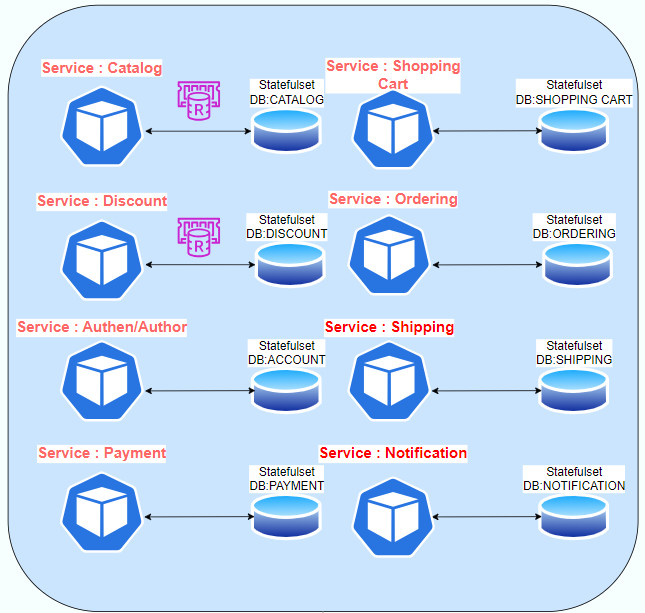
\includegraphics[scale = 0.7]{images/phat/DB_service.jpg}
    \vspace*{7mm}
    \caption{Database service}
    \end{center}
    \label{}
\end{figure}
\noindent Hệ thống có nhiều service nhỏ, mỗi service được build thành một docker image, sau đó dùng docker image này để deploy lên k8s với các pod bọc ngoài các container. Deployment là đơn vị quản lý trực tiếp các pod, đảm bảo tính availability và scalability. HPA sẽ kết nối tới deployment, có tác dụng thay đổi số bản sao của pod trong deployment dựa theo các metric – thông số của pod được đo đạc và xác định realtime. Dựa vào một hoặc một vài thông số này để autoscaling.
 \begin{figure}[H]
    \begin{center}
    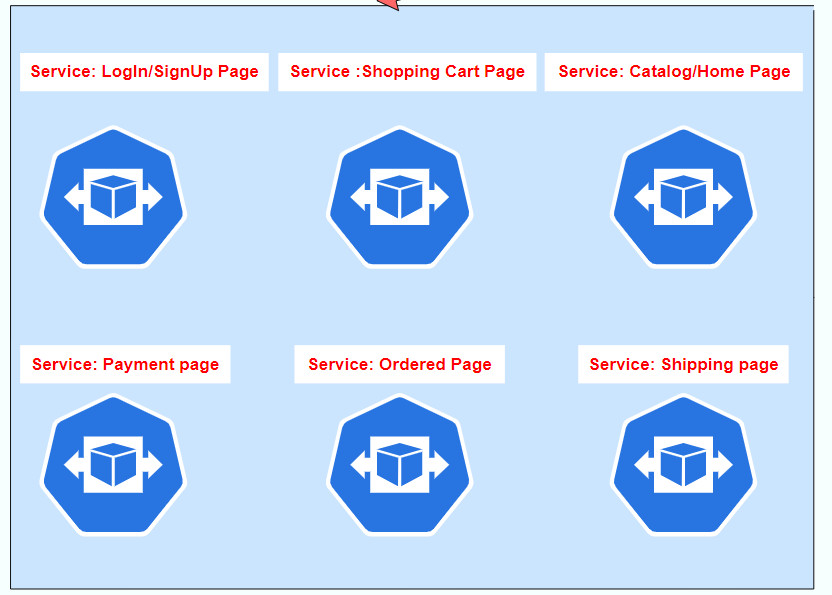
\includegraphics[scale = 0.6]{images/phat/frontend-service.jpg}
    \vspace*{7mm}
    \caption{Front-end service}
    \end{center}
    \label{}
\end{figure}
 \begin{figure}[H]
    \begin{center}
    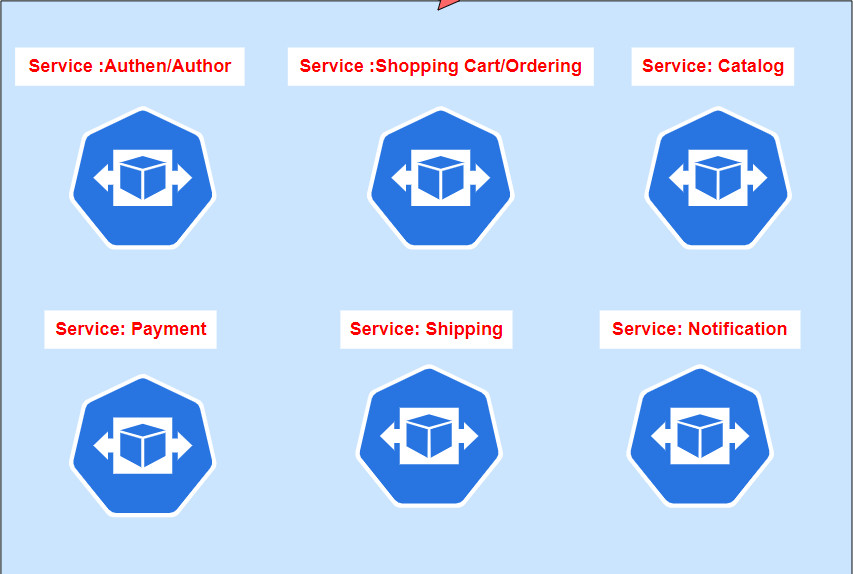
\includegraphics[scale = 0.6]{images/phat/backend-service.jpg}
    \vspace*{7mm}
    \caption{Back-end service}
    \end{center}
    \label{}
\end{figure}

\noindent Mỗi microservice sẽ có một service k8s (Trong môi trường Kubernetes, "service" là một đối tượng trừu tượng giúp liên kết các microservices và cung cấp một cổng vào các ứng dụng chạy trong môi trường container) để làm endpoint truy cập đến các pod do địa chỉ IP các pod thay đổi trong khi đó địa chỉ IP của service thì lại không đổi. Ngoài ra, chúng ta có thể dùng service name để gọi thay IP cho mỗi microservice. Service name này dùng để gọi nội bộ giữa các service trong cluster. Khi triển khai ứng dụng lên cloud hệ thống sẽ cung cấp thêm các master node để đảm bảo tính availability, bên cạnh đó, chúng ta cũng có thể tận dụng được firewal hay các traffic rule để đảm bảo tính security và chống DDoS.

\noindent Hệ thống còn dùng thêm một tính năng khác của K8s là Cluster Autoscaler để tự động mở rộng hoặc thu hẹp kích thước của một cluster Kubernetes bằng cách thêm hoặc giảm số lượng các node (máy ảo hoặc máy vật lý) trong cluster nhằm duy trì một số lượng node đủ để chứa tất cả các Pods đang chạy trong cluster mà không gây lãng phí tài nguyên.
 \begin{figure}[H]
    \begin{center}
    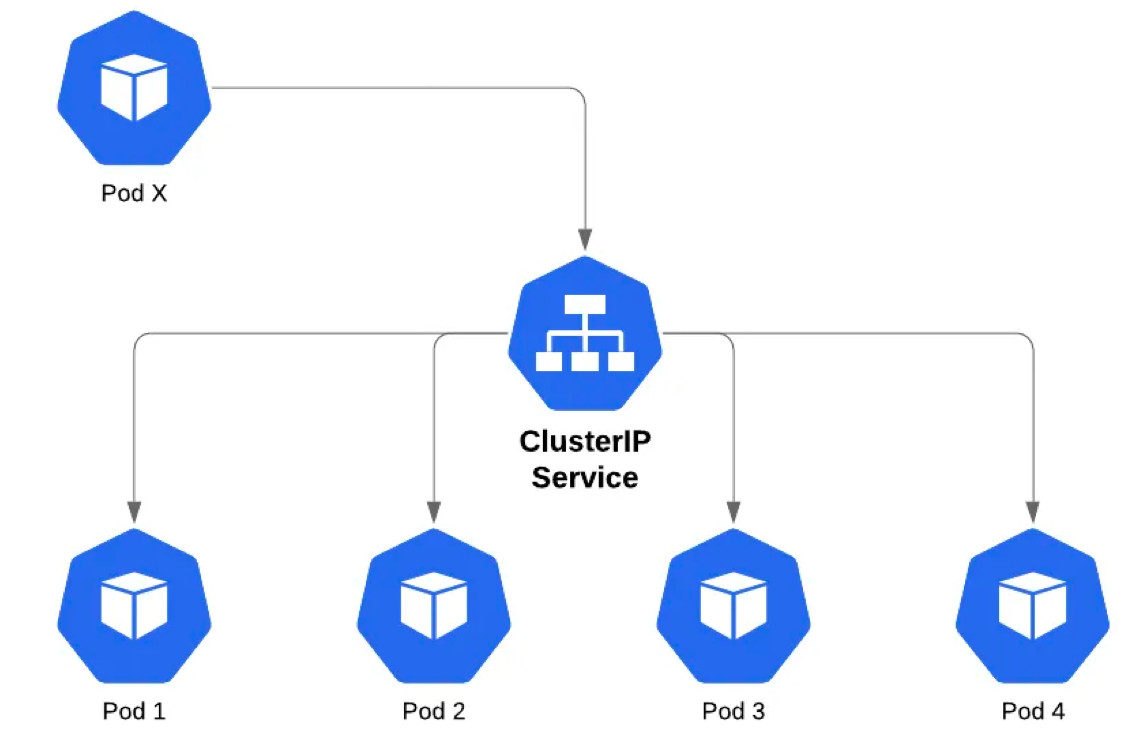
\includegraphics[scale = 0.25]{images/phat/service-cluster.jpg}
    \vspace*{7mm}
    \caption{Kubernetes Service}
    \end{center}
    \label{}
\end{figure}
\section{Thiết kế Database}
\textbf{Thiết kế Database cho chức năng hiển thị sản phẩm}
 \begin{figure}[H]
    \begin{center}
    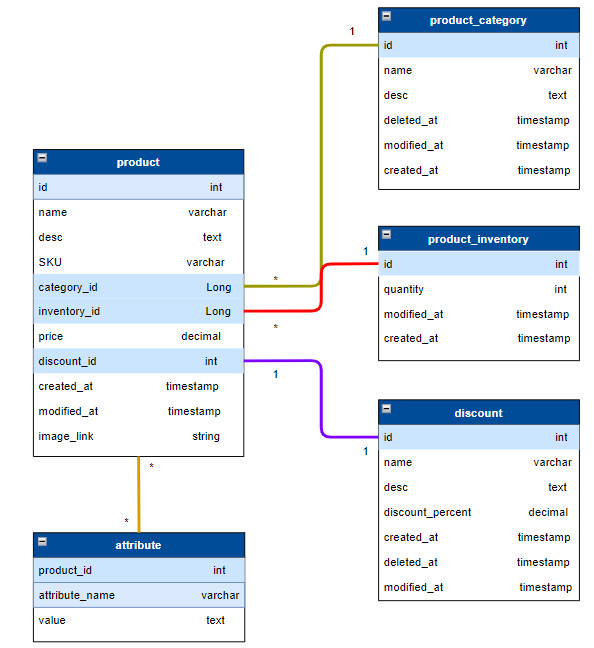
\includegraphics[scale = 0.8]{images/phat/DB_catalog.jpg}
    \vspace*{7mm}
    \caption{Database cho hiển thị sản phẩm}
    \end{center}
    \label{}
\end{figure}
\textbf{\textit{Ghi chú:}}
\begin{itemize}
    \item [-] 1..*: Mối quan hệ 1-N.
    \item [-] 1..1: Mối quan hệ 1-1.
    \item [-] *..*: Mối quan hệ N-N.
\end{itemize}
\noindent{\textbf{Mô tả:}}\\
\noindent Cấu trúc database cho hiển thị danh sách sản phẩm gồm có 05 bảng dữ liệu:
\begin{itemize}
    \item [-] Bảng product: chứa thông tin chi tiết sản phẩm.
    \item [-] Bảng product\_category: chứa thông tin loại sản phẩm.
    \item [-] Bảng product\_inventory: chứa thông tin nơi lưu trữ sản phẩm.
    \item [-] Bảng discount: chứa thông tin về giảm giá.
    \item [-] Bảng attribute: chứa thông tin về thuộc tính của sản phẩm.
\end{itemize}
